\documentclass[[a4paper,11pt]{article}
\renewcommand{\rmdefault}{ptm}
\usepackage[scaled=0.92]{helvet}
\usepackage{courier,xcolor,colortbl,listings,parskip,graphicx,fancyvrb,fancyhdr,lastpage}
\usepackage{float,framed}
\normalfont
\usepackage[T1]{fontenc}
\setlength{\parskip}{7pt}
\usepackage[toc,page]{appendix}
\usepackage[hmargin=2.5cm,vmargin=2cm]{geometry}
\usepackage[utf8]{inputenc}
\usepackage[brazil]{babel}
\pagestyle{fancy}
\setlength{\headheight}{120pt}
\setlength{\headsep}{30pt}
\setlength{\textheight}{550pt}
\renewcommand{\headrulewidth}{0pt}
\lhead{}
\rhead{}
\chead{
\includegraphics{brasao.jpg}\\
        \large \textbf{PRESIDÊNCIA DA REPÚBLICA}\\
        \large SECRETARIA-GERAL\\
        \large Secretaria-Executiva}
\cfoot{}
\rfoot{\thepage /\pageref{LastPage}}
\hyphenation{par-ti-ci-pa-ção}
\bibliographystyle{ieeetr}

\newcommand{\MyName}{Daniela Soares Feitosa}
\newcommand{\MyEmail}{daniela@colivre.coop.br}
\newcommand{\ContractNumber}{2013/000292}
\newcommand{\ProjectCode}{Projeto PNUD BRA/12/018}
\newcommand{\NomeSecretaria}{Secretaria Geral da Presidência da República}
\newcommand{\SiglaSecretaria}{SG/PR}
\newcommand{\ProductNumber}{05}
\newcommand{\ProductDescription}{Documento com proposta para 
desenvolvimento do código do tema das
comunidades contendo exemplos e códigos.}
\newcommand{\MesEntrega}{Maio de 2014}
\newcommand{\DiaEntrega}{26}

\begin{document}
\lstset{language=Ruby}
\definecolor{light-gray}{gray}{0.95}
\lstdefinestyle{codeFrame}{backgroundcolor=\color{light-gray},frame=lines}

\textbf{\ProjectCode \ -} \ProductDescription

\vspace{3cm}

\begin{minipage}{0.5\textwidth}
  \textbf{Consultora: \MyName}
  \newline
  \textbf{Contrato nº: \ContractNumber}
  \newline
  \textbf{Produto / nº: \ProductNumber}
\end{minipage}

\vspace{2cm}

\textbf{Assinatura do Consultor}

\begin{framed}
Local e data: Brasília/DF, \line(1,0){20} \ de \line(1,0){100} \ de 2014
\newline
\newline
Assinatura do Consultor: \line(1,0){300}
\end{framed}

\vspace{1cm}

\textbf{Assinatura do Supervisor}

\begin{framed}
Atesto que os serviços foram prestados conforme estabelecido no Contrato
de Consultoria.
\newline
\newline
Local e data: Brasília/DF, \line(1,0){20} \ de \line(1,0){100} \ de 2014
\newline
\newline
Assinatura e Carimbo: \line(1,0){300}
\end{framed}

\clearpage
\newcolumntype{g}{>{\columncolor{light-gray}}l}

\begin{center}
  \begin{tabular}{| g | p{10cm} |}
    \hline
    \textbf{Título} & \ProductDescription \\ \hline
    \textbf{Língua do documento} & Português - Brasil \\ \hline
    \textbf{Documentação de referência} & Português \\ \hline
    \textbf{Unidade responsável} & \NomeSecretaria \
(\SiglaSecretaria) \\ \hline
    \textbf{Criador} & \MyName - \MyEmail \\ \hline
    \textbf{Taxonomias} & Desenvolvimento \\ \hline
    \textbf{Data de aprovação} &  \\ \hline
    \textbf{Público} & \SiglaSecretaria, Parceiros e Sociedade
Civil \\ \hline
    \textbf{Faz parte do} & \ProjectCode \\ \hline
    \textbf{Em conformidade com a} & \NomeSecretaria \\ \hline
    \textbf{Documentos anexos} & Página da Comunidade OSC - Organizações da
Sociedade Civil; CSS do cabeçalho do tema de comunidade; Código javascript para
incluir uma classe identificadora; Código CSS para estilizar os blocos com o padrão
colorido \\ \hline
    \textbf{Revisado em} &  \\ \hline
  \end{tabular}
\end{center}

\clearpage

\tableofcontents
\clearpage
\listoffigures

\clearpage

\section{Introdução}

A participação social no Brasil representa princípio
jurídico-institucional
presente na Constituição Federal de 1988, que a definiu como forma de
afirmação da
democracia e da consolidação da cidadania. Ao incorporar esse princípio
como
referência para a gestão pública, o Governo Federal aprimora os
processos de interação
do Estado com a sociedade e cria as condições institucionais para a
prática da
democracia participativa. Com isso, verifica-se que, além da crescente
participação
social nas decisões governamentais, as políticas públicas ganham maior
legitimidade,
uma vez que expressam as atuais condições socioeconômicas e culturais da
população
brasileira em suas diferentes realidades regionais.

Na estrutura administrativa do Poder Executivo Federal, cabe à
Secretaria-Geral
da Presidência da República (SG/PR) a função de intermediar as relações
do Governo
com as entidades da sociedade civil, conforme competências definidas
pela Lei
10.683/2003 e pelo Decreto no. 7.688/2012. Assim, a SG/PR é órgão
incumbido de
assessorar diretamente a Presidenta da República e os órgãos e entidades
do Governo
Federal no relacionamento e na articulação com os movimentos sociais, o
que inclui a
criação e a implementação de canais que assegurem a consulta e a
participação popular
na discussão e na definição da agenda prioritária do país.

O Brasil tem um rico histórico de efetivação da democracia
participativa, sendo
reconhecido mundialmente. Os instrumentos institucionalizados como
conselhos de
políticas públicas e conferências nacionais foram profundamente
ampliados na última
década, contando com um legado volumoso de práticas e realizações. A
maioria dos
programas de governo já conta com participação social prevista em pelo
menos uma de
suas etapas. As práticas trazidas pelas novas mídias e pela cultura
digital podem
interagir nesses espaços fortalecendo, ampliando e aprofundando a
democracia
participativa, já na abordagem do novo século, pós redes sociais
digitais.

Incentivando os atores a conectar perfis, blogs e demais instâncias de
produção
de conteúdo na rede, o Portal de Participação Social poderá se
estabelecer como um
repositório agregador do conhecimento sobre participação social hoje
disperso na
internet e nas instâncias governamentais. A partir de uma interface
clara que possibilite
a navegação pelos temas, o Portal de Participação Social pode ser um
espaço onde os
diferentes agentes de governo, movimentos, organizações e cidadãos em
geral
encontrarão solo fértil e facilitado para o exercício da pesquisa e do
diálogo.

Tendo por base a premissa de que a incursão e abertura de canais de
acesso ao
poder público na rede aumenta o conhecimento das ações do governo e
diminui as
barreiras para participação de cidadãos, entidades e movimentos, esse
projeto visa a
construção de um conjunto de ferramentas que poderão ser utilizadas por
gestores e
servidores para proporcionar novas formas de participação a serem
apropriadas pela
cidadania. Além disso, esse portal também buscará dar evidência às
formas de
participação existentes no sentido de contextualizar, organizar e
facilitar o acesso do
cidadão às formas de incidir nas diversas etapas das políticas públicas
do governo
brasileiro.

\section{Apresentação}

Este documento é parte da consultoria para o projeto
\textbf{Desenvolvimento de Metodologias de Articulação e Gestão de
Políticas Públicas para Promoção da Democracia Participativa}
(BRA/12/018), firmado entre a Secretaria-Geral da Presidência da República
(SG/PR) e o Programa das Nações Unidas para o Desenvolvimento (PNUD).
A consultoria tem como objetivo a especificação da construção dos códigos das
metodologias de organização da informação e interação participativa do
portal da participação social.

O presente documento apresenta a proposta para
desenvolvimento do código do tema das comunidades contendo exemplos e códigos.
Essa proposta está configurada como produto 5 da consultoria técnica.

Neste documento será apresentada a especificação e
modelagem para desenvolvimento do código necessário para aplicação do
tema de comunidades criadas no portal Participa.br como definido 
pela equipe do projeto Participa.br em parceria com a equipe da
Secretaria-Geral da Presidência da República responsável 
pela agenda do Marco Regulatório das Organizações da Sociedade Civil (MROSC).

O Portal de Consulta Pública utiliza o software livre Noosfero,
plataforma web para redes sociais, então o código produzido deverá ser público
e divulgado para a comunidade e para os que desenvolvem e se utilizam do
software.

\section{Personalização de comunidades no Participa.br}

No Noosfero, plataforma base do Participa.br, o foco é rede social para
produção e publicação de conteúdo na Internet. Cada perfil criado na plataforma
tem também a função de site e funciona como uma página personalizável.

Os perfis do tipo "Comunidade" criados no Participa.br servirão como um 
espaço onde os diferentes agentes de governo, movimentos, organizações e 
cidadãos em geral se organizarão para compartilhar interesses, preferências
e, utilizando o conjunto de ferramentas disponíveis, proporcionar novas 
formas de participação a serem apropriadas pela cidadania.

Criada por uma pessoa e mantida por uma ou mais, o perfil "Comunidade" é 
caracterizado por um coletivo de usuários que tem como objetivo agregar pessoas
em torno de interesses comuns. 

A personalização de uma Comunidade no Participa.br envolve quatro itens principais:

\subsection{Alteração de template}

Acessando a seção "Editar Aparência" pelo painel de controle da comunidade 
(Figura~\ref{fig:editar-template}), o administrador da comunidade poderá escolher
como será a organização de colunas da página.

As imagens nessa tela tentam mostrar como ficará a organização das colunas da
página. O retângulo mais largo representa a área com o conteúdo principal da
página e os outros retângulos representam as colunas para inserção de blocos.

Todas as opções disponíveis inclui o bloco que irá mostrar o conteúdo principal
da página. A escolha do administrador nessa seção é sobre a presença, quantidade
e posição das colunas para blocos.

\begin{figure}[h]
\center
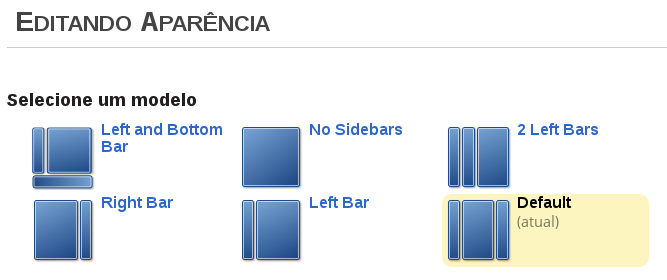
\includegraphics[scale=0.5]{editar-template.png}
\caption{Tela para escolha de template}
\label{fig:editar-template}
\end{figure}

\subsection{Organização de blocos}

Na seção "Editar blocos laterais" do painel de controle da comunidade 
(Figura~\ref{fig:editar-blocos}), o administrador visualizará as colunas da
página de acordo com o template configurado.

Clicando no botão "Adicionar blocos" o administrador poderá escolher quais
blocos serão inseridos na página. Cada bloco tem uma funcionalidade específica e
deve ser escolhido de acordo com o objetivo da comunidade.

\begin{figure}[h]
\center
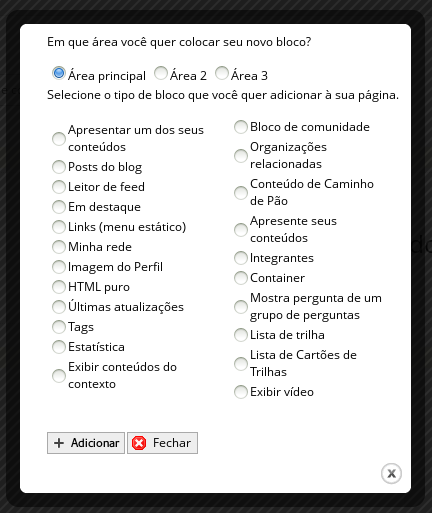
\includegraphics[scale=0.5]{editar-blocos.png}
\caption{Tela para adicionar blocos}
\label{fig:editar-blocos}
\end{figure}

\subsection{Edição de cabeçalho e rodapé}

Na seção "Editar Cabeçalho e Rodapé", o administrador pode alterar o que será
visualizado pelos usuários no topo e na parte inferior da sua comunidade. O
cabeçalho e rodapé é visível em todas as páginas da comunidade, portanto, deve
dar preferência por inserir conteúdos estratégicos. No cabeçalho, é
importante que seja inserido um banner sobre o objetivo da comunidade e no
rodapé, informações importantes e que devem ficar sempre visíveis.

\begin{figure}[h]
\center
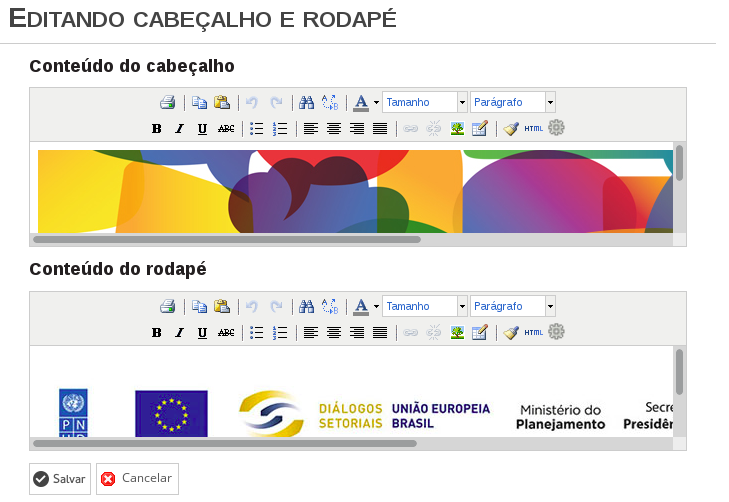
\includegraphics[scale=0.5]{editar-cabecalho-rodape.png}
\caption{Tela para edição de cabeçalho e rodapé}
\label{fig:editar-cabecalho-rodape}
\end{figure}

\subsection{Alteração do tema}

Também na seção "Editar Aparência" pelo painel de controle da comunidade 
(Figura~\ref{fig:editar-tema}), o administrador da comunidade poderá escolher
alguns temas que ficarão disponíveis para as comunidades.
Além dos temas disponíveis por padrão no Participa.br, é possível criar novos
temas para personalizar as comunidades.

\begin{figure}[h]
\center
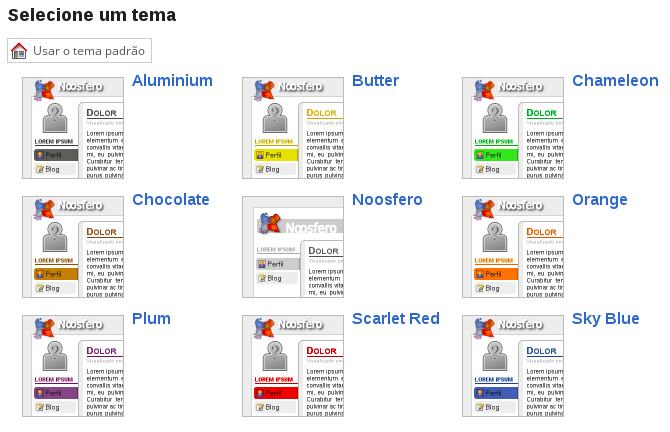
\includegraphics[scale=0.5]{editar-tema.png}
\caption{Tela para escolha de tema}
\label{fig:editar-tema}
\end{figure}

\section{Proposta para desenvolvimento do código do tema das 
comunidades contendo exemplos e códigos.}

Neste documento, é proposta uma nova opção de tema de comunidade que foi
utilizada na comunidade OSC (http://www.participa.br/osc) e pode ser aplicada em
outras comunidades no Participa.br.

As ideias que serviram como base para a definição da arquitetura de
informação e do tema de comunidade do portal de Consulta Pública foram
discutidas em reuniões com integrantes da Secretaria Geral da
Presidência da República (SG/PR) em parceria com os responsáveis pela agenda do
Marco Regulatório das Organizações da Sociedade Civil (MROSC).

O gráfico do layout para o tema foi desenvolvido por consultores vinculados à
equipe da agenda do MROSC e aprovado pela equipe gestora do projeto. O tema padrão
pode ser visualizado no
Anexo~\ref{Att:PaginaComunidade}.

Para a codificação do tema foi utilizado como base o tema "Conference". Esse
tema foi produto de uma consultoria que integra o processo de preparação da
Conferencia Nacional sobre Migrações e Refúgio (COMIGRAR).
O tema "Conference" foi implementado por Valéssio Soares de Brito em parceria
com o Laboratório Avançado de Produção, Pesquisa e Inovação em Software da UNB -
Gama, coordenado pelo professor Dr. Paulo Roberto Miranda Meirelles. O tema está
disponível no repositório oficial do projeto: 
https://gitlab.com/participa/conference-theme .

O ideal é que o Participa.br/Noosfero tenha uma estrutura para que os próprios
usuários possam criar e aplicar os temas nas suas comunidades. Enquanto isso não
é desenvolvido, todos os temas do Participa.br devem ser públicos e disponíveis
no repositório oficial do projeto (https://gitlab.com/participa/). A inclusão
dos temas no repositório facilita a manutenção e evolução por outras pessoas, já
que garante a possibilidade de contribuição e o controle de versão dos arquivos.

\subsection{Cabeçalho da comunidade com a identidade visual do Portal}

\begin{figure}[h]
\center

\includegraphics[scale=0.35]{cabecalho-reduzido.png}
\caption{Cabeçalho do portal reduzido}
\label{fig:cabecalho-reduzido}
\end{figure}

\begin{figure}[h]
\center
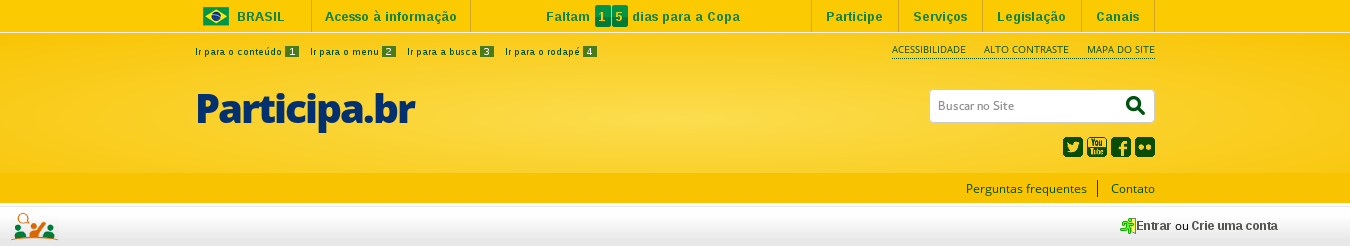
\includegraphics[scale=0.35]{cabecalho.png}
\caption{Cabeçalho do portal}
\label{fig:cabecalho}
\end{figure}

O cabeçalho do Portal de Participação Social do Governo Federal na internet
segue o modelo utilizados em outros sites do Governo Federal.

À esquerda constam os links para acesso rápido à algumas
seções da página e o nome do Portal.
À direita constam os links de acessibilidade, mapa do site, campo de
busca, links para outras redes sociais e links de perguntas e contato do
Portal.

Para manter a identidade visual do Portal nas comunidades, todas as comunidades
irão apresentar o cabeçalho padrão. Ao acessar uma comunidade, o usuário verá
ema versão reduzida do cabeçalho para permitir um espaço maior para o conteúdo
criado na comunidade (Figura~\ref{fig:cabecalho-reduzido}). Quando o usuário
passar o mouse sobre a barra superior, o cabeçalho se expandirá, mostrando o
cabeçalho completo (Figura~\ref{fig:cabecalho}).  

O código CSS que mostra o cabeçalho completo ao passar o mouse sobre a barra do Portal pode ser visualizado no
Anexo~\ref{Att:CabecalhoComunidade}.

\subsection{Cabeçalho e rodapé da comunidade}

\begin{figure}[h]
\center

\includegraphics[scale=0.5]{banner-destaque.png}
\caption{Banner de destaque da comunidade}
\label{fig:banner-destaque}
\end{figure}

\begin{figure}[h]
\center

\includegraphics[scale=0.5]{logos-apoiadores.png}
\caption{Banner com logomarcas dos apoiadores}
\label{fig:logos-apoiadores}
\end{figure}

O banner no cabeçalho (Figura~\ref{fig:banner-destaque}) e rodapé
(Figura~\ref{fig:logos-apoiadores}) da comunidade são compostos por imagens que
possuem dimensões: 960x200px e 960x125px respectivamente, com imagens
no formato JPG ou PNG, contendo a identidade visual e logo da comunidade no
cabeçalho e as logos de parceiros e realizadores no rodapé.

As imagens utilizadas como exemplos foram utilizadas na comunidade OSC
(http://www.participa.br/osc). Ao utilizar o tema em outra comunidade, as
imagens deverão ser alteradas para se adequar ao conteúdo das comunidades,
respeitando as dimensões informadas acima. 

\subsection{Bloco de Links}

\begin{figure}[h]
\center
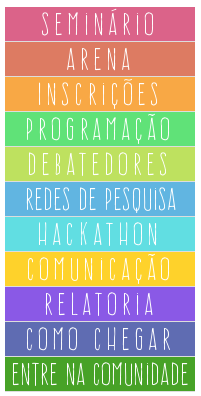
\includegraphics[scale=0.4]{bloco-links.png}
\caption{Bloco de links}
\label{fig:bloco-links}
\end{figure}

O Noosfero já possui um bloco de links onde podem ser inseridos quaisquer links
que o administrador da comunidade desejar. Para esse tema, o bloco de links
(Figura~\ref{fig:bloco-links}) foi configurado como um menu com os principais
conteúdos da comunidade.

Seguindo o layout aprovado pela equipe, apenas o primeiro bloco de links da comunidade teria a
apresentação alterada em relação ao tema base "Conference". Para isso, foi
necessária a inclusão de um código javascript
(Anexo~\ref{Att:CodigoJsLinkColoridos}) para incluir uma classe "colored-links" ao redor
do bloco considerado como menu da comunidade. No arquivo CSS, as cores de cada
item do menu foram definidas como apresentado no
Anexo~\ref{Att:CodigoCSSLinkColoridos}.

Alguns itens do menu deveriam ter seu texto alterado quando 
o mouse passasse sobre ele (Figura~\ref{fig:bloco-links-hover}). Para isso, foi desenvolvido um código com javascript
que altera o texto a partir de uma lista dada e, nos casos que o texto tem a
largura maior que o texto original, o espaçamento das letras é reduzido para
evitar que o texto seja mostrado em mais de uma linha e cause estranhamento
visual.

\begin{figure}[h]
\center
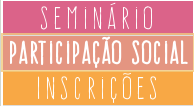
\includegraphics[scale=0.4]{bloco-links-hover.png}
\caption{Item do bloco de links com hover}
\label{fig:bloco-links-hover}
\end{figure}

\subsection{Menu para edição da comunidade}

\begin{figure}[h]
\center
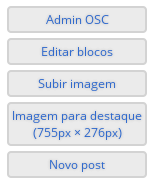
\includegraphics[scale=0.5]{menu-rapido.png}
\caption{Menu com atalhos para a administração da comunidade}
\label{fig:menu-rapido}
\end{figure}

Para facilitar a gestão do conteúdo e apresentação da comunidade, foi inserido
um menu com atalho para as principais seções de administração
(Anexo~\ref{Att:MenuAdministracao}). Esse menu só é
apresentado para os usuários logados e com papel de administrador na comunidade.

\subsection{Folha de Estilo - CSS}

O CSS é utilizada para definir a apresentação de documentos escritos em
uma linguagem de marcação, como HTML ou XML. Seu principal benefício é
prover a separação entre o formato e o conteúdo de um documento.

Ao invés de inserir a formatação diretamente no documento, é inserido
um link na página para o arquivo que contém as definições de estilo.

O CSS do tema pode ser visualizada no repositório oficial do Portal
( https://gitlab.com/participa/mrosc-theme/blob/master/style.css ). 

Como os temas do Portal estarão sempre em evolução, o arquivo com o CSS da
comunidade poderá ser atualizado para que os novos elementos
inseridos nas páginas sigam o padrão do tema.

\newpage

\section{Considerações finais}

Neste documento foi apresentada proposta do desenvolvimento do código do tema
das comunidades contendo exemplos e códigos.

O tema já está sendo utilizado numa comunidade ativa do Participa.br, a
comunidade OSC ( http://www.participa.br/osc ) e pode ser utilizada em outras
comunidades.

Com o objetivo de melhorar a usabilidade, apresentação ou atender às
necessidades das outras comunidades que a utilizarem, esse
tema poderá sofrer alterações.

Esse e todos os outros temas desenvolvidos para o Participa.Br ficarão
disponíveis no repositório oficial do projeto ( https://gitlab.com/participa/ ).

\vspace{1cm}

Sem mais nada a acrescentar, coloco-me à disposição.

\vspace{1cm}

\begin{minipage}{\textwidth}
  Brasília/DF, \DiaEntrega \ de \MesEntrega\\[1cm]
  \textbf{\MyName}\\
  \small Consultora do PNUD
\end{minipage}

\newpage
\appendix
\appendixpage
\section{Plugin class} \label{App:PluginCode}





\end{document}
